\section{Tutorial Ping Pong (Java and C)}
\label{sec:ping_pong_tutorial}

\subsection{Scope}

This tutorial describes how to create a simple hierarchical actor system of actors communicating via ports and bindings. 
Additionally you will use the Timing Service from the eTrice model library.
This tutorial can be done for the target languages Java or C.
For the Ping Pong scenario we want to create a model with a sender and a reveiver of a message. The receiver has to wait for the ping message from the sender, wait for a second and respond with a pong message.

The resulting Message Sequence Chart (MSC) at the end of this tutorial should look like this:

\includegraphics[width=0.7\textwidth]{images/015-msc.png}

We will take this MSC as specification for the desired behavior.

\subsection{Create the structure}

We start by opening the \emph{TemplateModel.room} from the template project as presented in Getting Started. As described previously \emph{topActor} is currently the only active actor. Furthermore the model provides a building kit for this tutorial, consisting of
\begin{itemize}
	\item ProtocolClass \emph{PingPongProtocol}: Defining the incoming message \emph{ping} and outgoing \emph{pong} according the specification
	\item ActorClass \emph{Receiver}: Defining a (regular) Port of type PingPongProtocol, which receives the incoming messages and sends the outgoing message. Additionally it has a reference to the \emph{TimingService}.
	\item ActorClass \emph{Sender}: Defining the \textbf{conjugated} Port of type PingPongProtocol, which handles the messages vice-versa
\end{itemize}

\begin{tabular}{c|c|c}
	\begin{lstlisting}[language=ROOM]
	ProtocolClass PingPongProtocol {
		incoming {
			Message ping()
		}
		outgoing {
			Message pong()
		}
	}
	\end{lstlisting} & 
	\begin{lstlisting}[language=ROOM]
	ActorClass Receiver {
		Interface {
			Port recvPort: PingPongProtocol
		}
		Structure {
			external Port recvPort
			SAP timingService: PTimer
		}
		// ...
	}
	\end{lstlisting} &
	\begin{lstlisting}[language=ROOM]
	ActorClass Sender {
		Interface {
			conjugated Port sendPort: 
				PingPongProtocol
		}
		Structure {
			external Port sendPort
		}
		// ...
	}
	\end{lstlisting}
\end{tabular}


Note: The naming \emph{Sender} \emph{Receiver} is based on the first message exchange. \emph{Sender} is the first actor supposed to send a message (\emph{ping}) and \emph{Receiver} is the first actor to receive this message. Afterwards they change their roles and it is vice-versa for message \emph{pong}.

Remaining tasks:
\begin{itemize}
	\item creating actor hierarchic actor structure by using classes \emph{Sender} \emph{Receiver}
	\item establish port binding
	\item define the behavior of both actors
	\item use the \emph{TimingService}
	\item generate and run application, then verify resulting MSC
\end{itemize}

We are going to create hierarchic actor structure and \emph{TopActor} will functions as a pure container actor. Thus its current state machine is obsolete, we can ignore or delete it.

We continue to add the actors graphically and open the structure diagram of \emph{TopActor} by right-click in the Outline View on \emph{TopActor -> Edit Structure}.

\includegraphics[width=\textwidth]{images/015-edit-structure-top.png}

Drag and Drop an \emph{ActorRef} from the \emph{Palette} within the borders and name the new actor reference \emph{sender} and set the type to ActorClass \emph{Sender}. Repeat the step for the \emph{receiver}. 

\includegraphics[width=.8\textwidth]{images/015-add-sender.png}

Finally we connect the ports of both actors using the \emph{Binding} tool in the \emph{Palette}. Drag a connection between the two port to establish a Binding.

\includegraphics[width=.8\textwidth]{images/015-add-binding.png}

\subsection{Implement the Behavior}

We will implement two finite state machines (\emph{FSM}s) to define the event driven behavior of the actors  \emph{Sender} and \emph{Receiver}.

Before you start with the implementation, have a look at the MSC with the specification of the behavior.

Lets start with the \emph{Sender}. Right click to \emph{sender} \emph{Open Ref Behavior} and in the structure diagram of \emph{TopActor}.

\includegraphics[width=.6\textwidth]{images/015-open-behavior-sender.png}

According to our specification:
\begin{quote}
	 \emph{Sender} initially should send the message \emph{ping} and then take a state named \emph{sendingPing}. After receiving the message \emph{pong} it should remain in a state named \emph{receivedPong}.
\end{quote}

Drag and Drop the \textit{Initial Point} and a \textit{State} into the diagram. The latter causes the opening of the dialog \emph{Edit State}, in which we type the name \emph{sendingPing} and specify the entry code \verb|senderPort.ping();|. Note the content assist is activated by pressing CTRL+Space.

\includegraphics[width=.8\textwidth]{images/015-edit-sending.png}

In the same manner we create a second \emph{State} named \emph{receivedPong} but without any action.
 
Use the \textit{Transition} tool to draw the initial transition to \textit{sendingPing}. The dialog \emph{Edit Transition} will open and we just click \emph{OK} as no action is required. Note that initial transitions do not have any trigger events.

Again draw a transition from \textit{sendingPing} to \textit{receivedPong}. In the dialog for this transition we set the trigger event to message \emph{pong} of port \emph{sendPort} in the top right corner.

\includegraphics[width=\textwidth]{images/015-edit-transition-pinger.png}

At this point the behavior of \emph{Sender} is complete and should look like this:

\includegraphics[width=.8\textwidth]{images/015-sending-ping-fsm.png}


We turn our attention to actor \emph{Receiver} and open its state machine diagram.

According to the specification:

\begin{quote}
	\emph{Receiver} initially should wait for the message \emph{ping}. After a short time the message \emph{pong} should be sent back.
\end{quote}

We create the states \emph{waitingForPing}, \emph{receivedPing} and \emph{sendingPong} plus the initial transition.

We draw a transition from \emph{waitingForPing} to \emph{receivedPing} and select as trigger event the message \emph{ping} of port \emph{recvPort}.

\includegraphics[width=.5\textwidth]{images/015-transition-ping.png}

In the entry code of the state \emph{receivedPing} we start the timeout by sending the message \emph{startTimeout(500)} (time unit is ms) to the \emph{timingService} port:
\begin{quote}
\verb|timingService.startTimeout(500);|
\end{quote}

We draw a transition from \emph{receivedPing} to \emph{sentPong}. The event trigger is the respond \emph{timeout} of the timing service.

\includegraphics[width=.5\textwidth]{images/015-transition-timeout.png}

In the entry code of the state \emph{sentPong} we send the message \emph{pong} back to the \emph{Sender}: \verb|recvPort.pong();|

Now the behavior of \emph{Receiver} is complete, too. It should look like this:

\includegraphics[width=.8\textwidth]{images/015-sending-pong-fsm.png}

The PingPong model is done now. You can generate, compile and run it as described in \emph{Hello World for C} or \emph{Hello World for Java}. The generated MSC in folder \emph{log} should show the same MSC we used to specify the behavior at the beginning of this tutorial.

\includegraphics[width=.7\textwidth]{images/015-msc.png}

\subsection{Summary}

Within this tutorial you have learned how to create a FSM with transitions triggered by incoming messages. You have used entry code to send messages and have used the timing service from the model library. You are now familiar with the basic features of \eTrice{}. Further tutorials and examples will take this knowledge as a precondition.
